\label{chapter:used-molecules}
The following molecules have been used to conduct experiments. Images show the molecules in an orthographic projection. We will utilize porphyrine derivatives (\autoref{section:TBP}), functionalized pyrene molecules (\autoref{section:pyrene}), helicene species (\autoref{section:helicene}) and coronene (w\/o central borazine functionalization, see \autoref{section:HBC}).

All the depicted molecules are modeled in Hyperchem\cite{_hyperchemtm_1111} and calculated for optimized geometry with the AM1+ method. Afterwards their positions are exported and remodeled in blender. Note that this does not change their geometry. It is only for better control of the output (faster and more accurate model building especially in 3D) and for aesthetic reasons.

%%%%%%%%%%%%%%%%%%%%%%%%%%%%%%%%%%%%%%%%%%%%%%%%%%%%%%%%%%%%%%%%%%%%%%%%%%%%%%%%%%%%%%%%%%%
%%%%%%%%%%%%%%%%%%%%%%%%%%%%%%%%%%%	pyrenes   %%%%%%%%%%%%%%%%%%%%%%%%%%%%%%%%%%%%%%%%%
\subsection{Pyrene: Pyridilethynyl functionalized pyrenes}
\label{sec:pyrene}\index{molecules!Pyrene}
\begin{itemize}
	\item[tetra-pyrene:] 1,3,6,8-Tetra(4-Pyridylethynyl)pyrene
	\item[cis-pyrene:] 1,8-Bis(4-Pyridylethynyl)pyrene
	\item[trans-pyrene:] 1,6-Bis(4-Pyridylethynyl)pyrene
\end{itemize}

\begin{figure}[h!]
	\begin{center}
		\subfigure[Tetra-configuration]{
			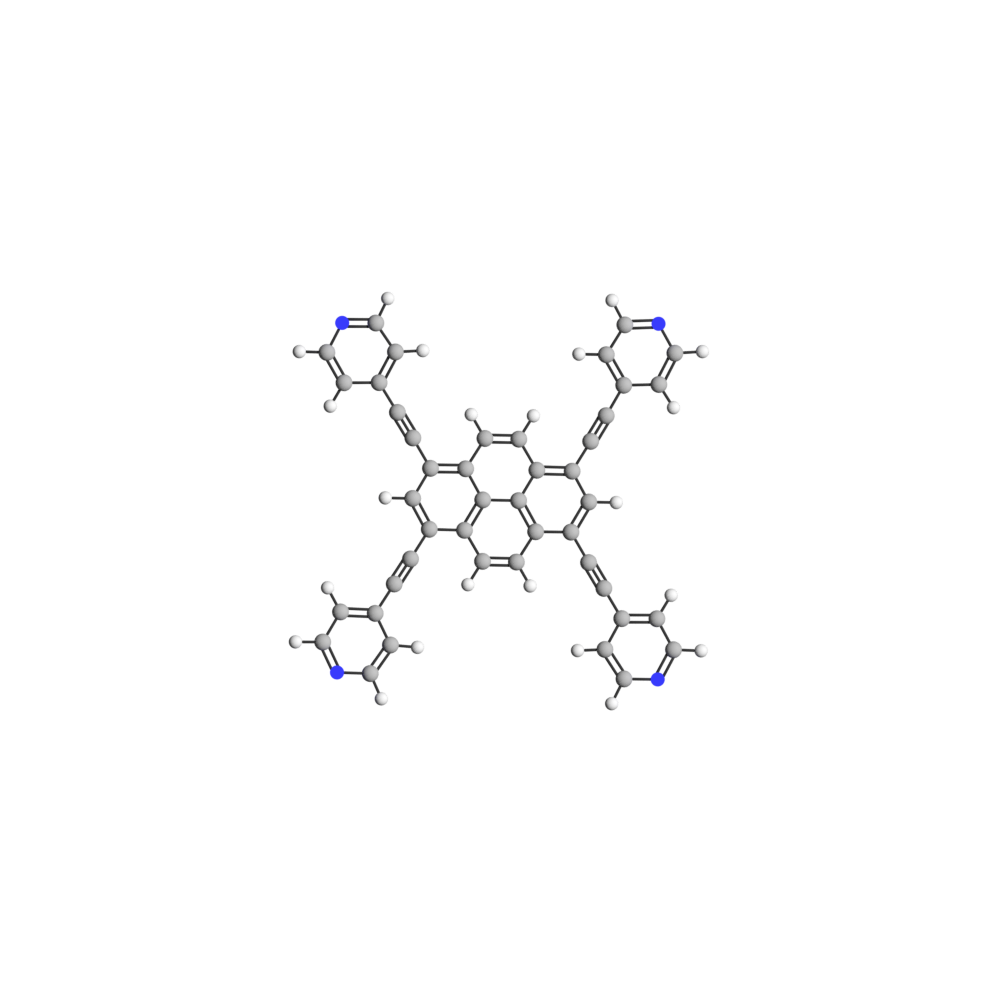
\includegraphics[width=0.3\textwidth]{./images/molecules/pyrene-tetra}
			\label{fig:pyrene-tetra}
		} 
		\subfigure[Trans-configuration]{
			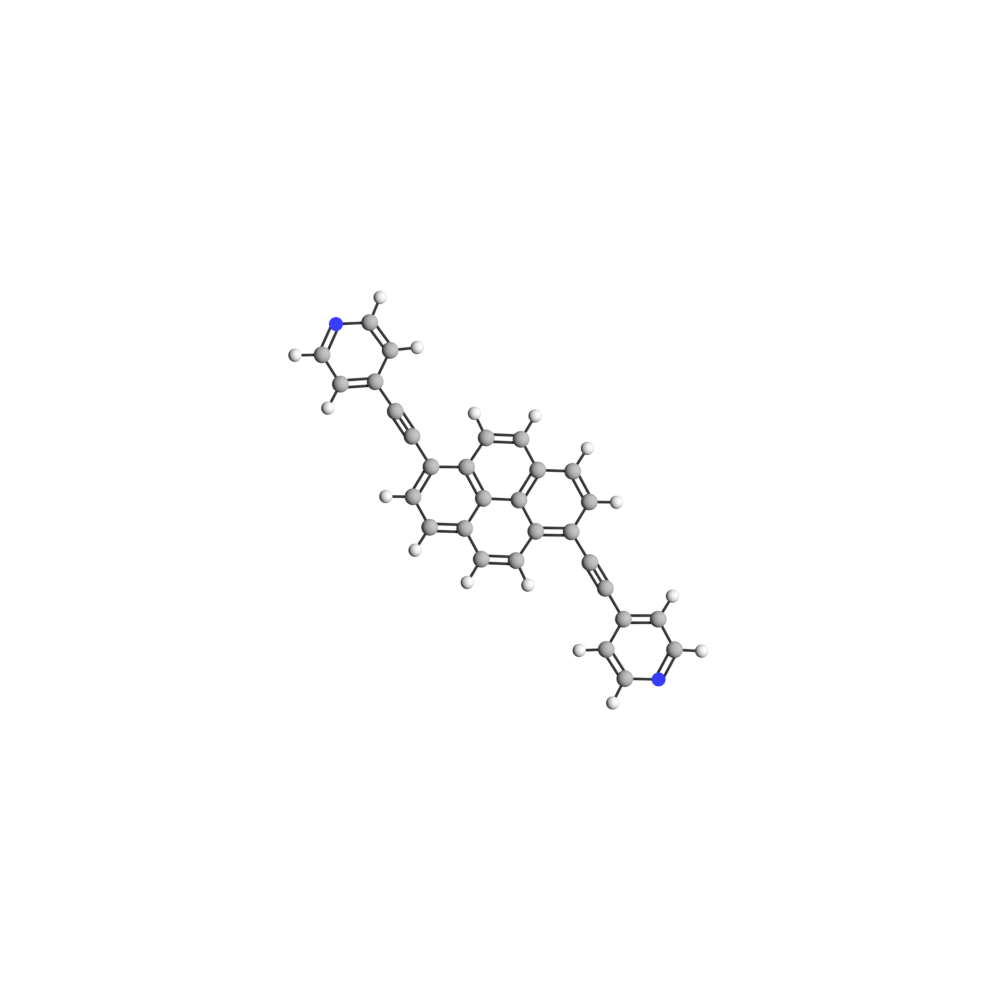
\includegraphics[width=0.3\textwidth]{./images/molecules/pyrene-trans}
			\label{fig:pyrene-trans}
		} 
		\subfigure[Cis-configuration]{
			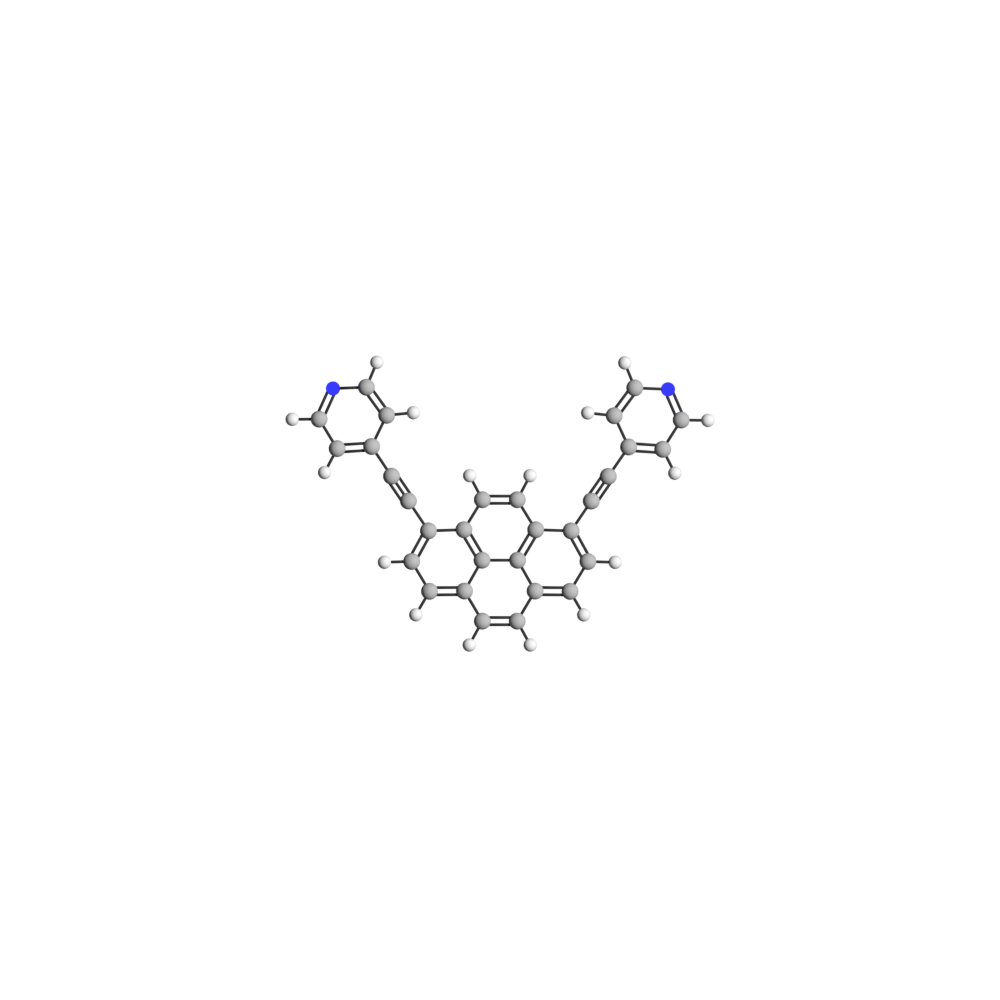
\includegraphics[width=0.3\textwidth]{./images/molecules/pyrene-cis}
			\label{fig:pyrene-cis}
		}
	\end{center}
	\caption{Pyridyl-Pyrene molecules in trans- \subref{fig:pyrene-trans} and cis- \subref{fig:pyrene-cis} and tetra- \subref{fig:pyrene-tetra} configuration}
	\label{fig:pyrene}
\end{figure}

Pyrene molecules, first investigated in 1973 \cite{khan_electronic_1973}, are 4 ortho-fused carbon rings to result in a rhombic structure. As many other $\pi$ conjugated systems they show interesting optoelectronic properties \cite{Crawford_experimental_2011, Lee_enhanced_2012, Feng_functionalization_2016, Maeda_alkynylpyrenes_2006, Kurata_donor_2017} and their assembly was investigated \cite{pham_self-assembly_2014, matena_aggregation_2010, della_pia_anomalous_2014, pham_comparing_2016}. Here they are used to investigate the influence of the number and position of functional groups on these properties. The very same species have been investigated on Cu(111) albeit data adsorbed on \textit{h}-BN/Cu(111) was lacking up to this point. The nano-pattering effect of the \textit{h}-BN substrate is used here to modulate the wide band gap of the species and therefor their optical properties.

\textcolor{red}{\textbf{DIPOLE / CHIRALITY / Ref section}}
%%%%%%%%%%%%%%%%%%%%%%%%%%%%%%%%%%%%%%%%%%%%%%%%%%%%%%%%%%%%%%%%%%%%%%%%%%%%%%%%%%%%%%%%%%%
%%%%%%%%%%%%%%%%%%%%%%%%%%%%%%%%%%%	HBBNC + HBC   %%%%%%%%%%%%%%%%%%%%%%%%%%%%%%%%%%%%%%%%%
\subsection{Coronene: HBBNC and HBC}
\label{sec:hbc}\index{molecules!Coronene}
\begin{itemize}
	\item[HBC:] 2,8,14-trixylyl-hexabenzocoronene	
	\item[HBBNC:] 2-8-14-trixylyl-hexaphenyl borazinocoronene
\end{itemize}

\begin{figure}[h!]\centering
\subfigure[HBC]{
	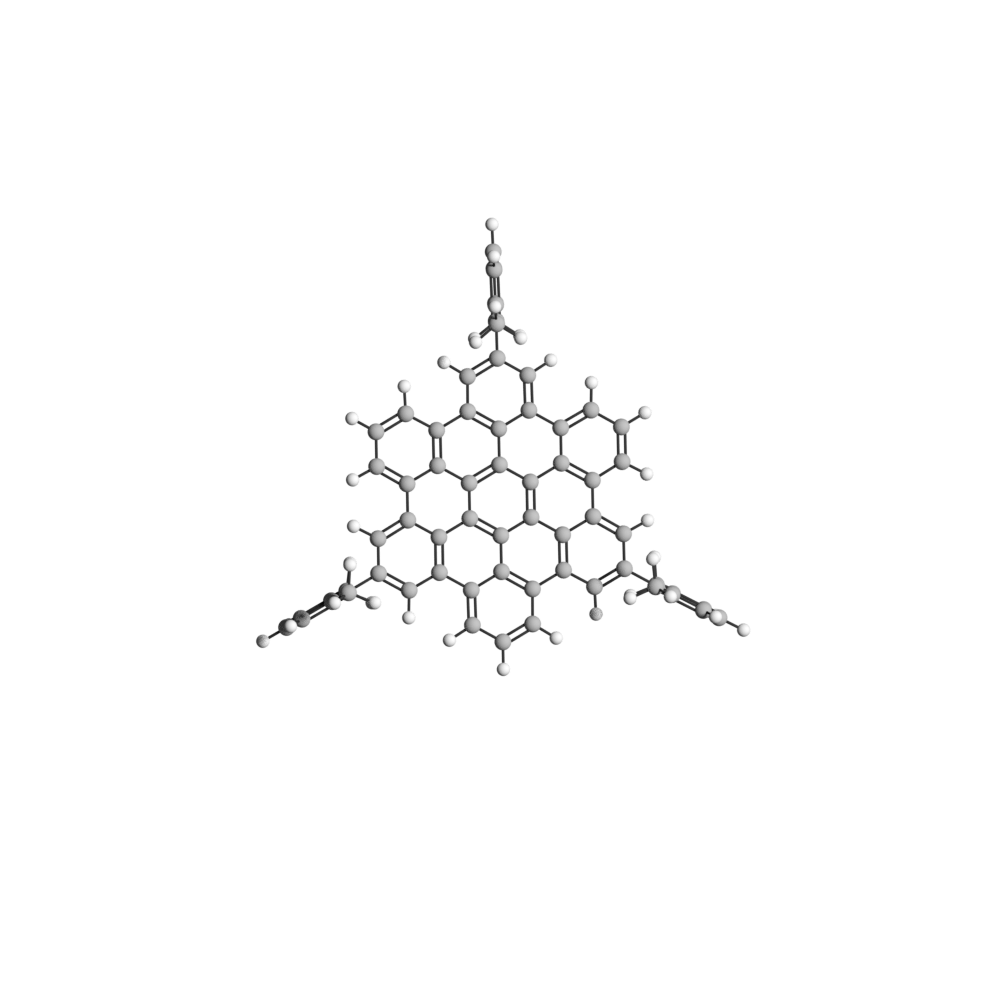
\includegraphics[width=0.3\textwidth]{./images/molecules/HBC}
	\label{fig:HBC}
} \quad
\subfigure[HBBNC]{
	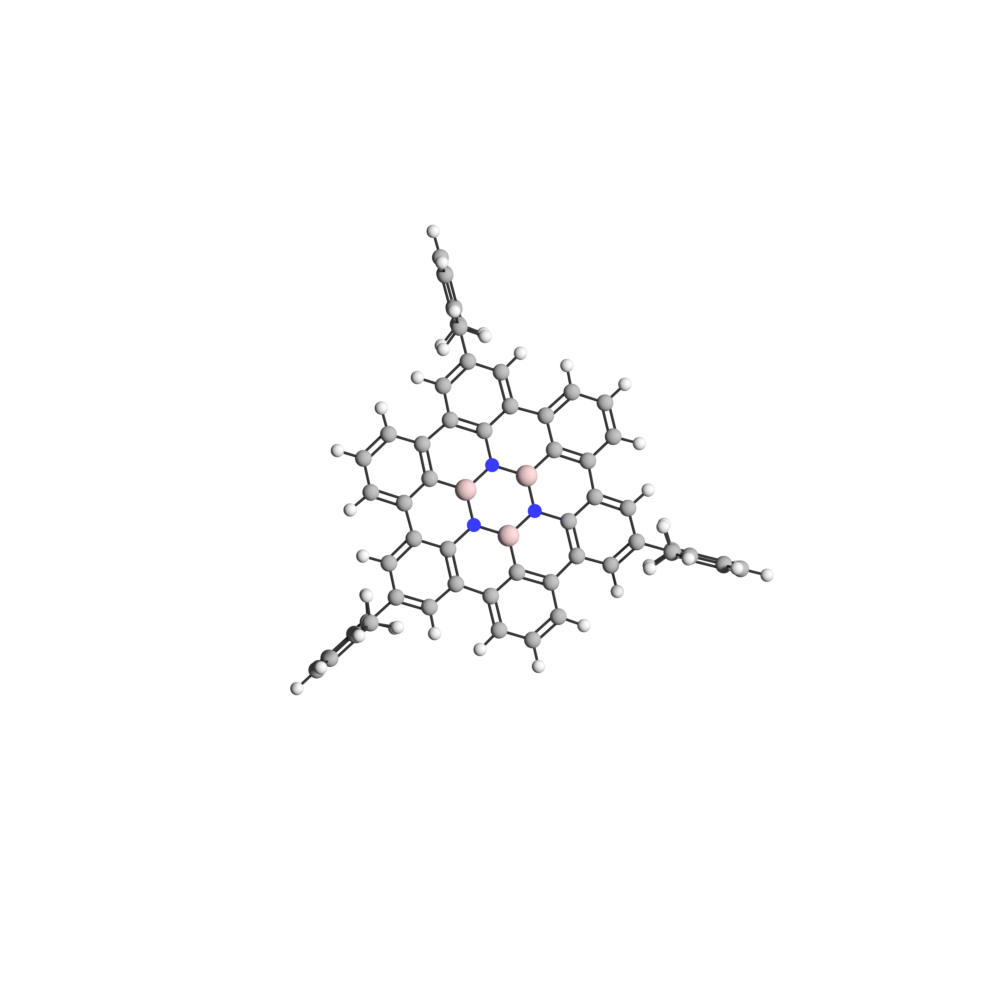
\includegraphics[width=0.3\textwidth]{./images/molecules/HBBNC}
	\label{fig:HBBNC}
}
	\caption{\subref{fig:HBC} HBC and \subref{fig:HBBNC} HBBNC}
	\label{fig:HBBNC+HBC}
\end{figure}

While in 2015\cite{Krieg_construction_2015} and 2016 \cite{Ciccullo_Quasi-Free-Standing_2016} hexy-peri-Hexabenzoborazino coronene (HBBNC) was synthesized, its bad solubility prohibited experiments. In 2017 the synthesis \cite{dosso_synthesis_2017} of a soluble, BN-doped coronene derivative by substitution of the central carbon ring was successful. 
\begin{wrapfigure}{R}{5cm}\centering
	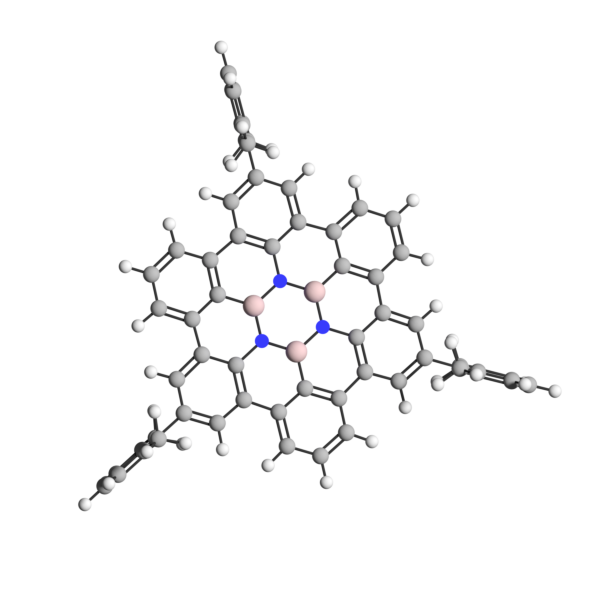
\includegraphics[angle=90,width=5cm]{./images/molecules/max-zoom/HBBNC-600}
	\caption{HBBNC}
	\label{fig:HBBNC-molecule}
\end{wrapfigure}

HBC and HBBNC are modifications of coronene. First, for both species six benzo groups are added to form a larger molecular backbone. For both species three 2,6-Dimethylphenyl groups are added to extend the molecule that now resembles a triangular footprint. While HBC features a central carbon ring, HBBNC is functionalized with a central borazine ring instead. Here the central $(BN)_3$ core is oriented to point all nitrogen atoms towards the leg functionalization.

Both species have the same number of atoms and molecular weight. The difference between both becomes apparent when electronic properties are compared (in gas phase).

The regular covalent sp2 hybridization results in an evenly distributed electron density in HBC where the central region of the molecule shows considerable depletion. Changing the central carbon ring to a borazine ring changes the electron density. Now electrons are redistributed from the coronene parts towards the central borazine ring. Because the bond between B and N shows an added ionic character the aromacity is interrupted and the extended electron pi system is altered. Comparable to the difference between graphene (perfect C-C bonds, conductor) and h-BN (Ionic B-N bonds, insulator) the band gap present for HBC is \SI{0.4}{\eV} smaller than for HBBNC, changing its optoelectronic properties. By using HBBNC the HOMO-LUMO band gap could be widened and shows blue-shifted emission properties\cite{dosso_synthesis_2017} compared to its all-carbon counterpart.

\begin{figure}[]\centering
	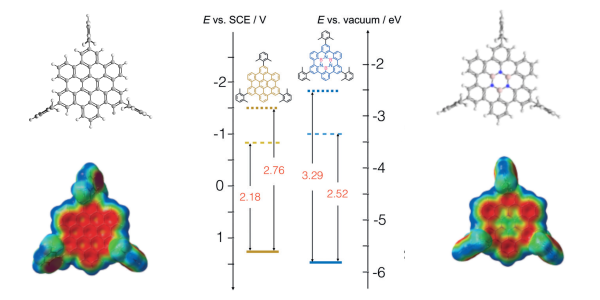
\includegraphics[width=\textwidth]{./images/dosso-combined}
	\caption{Taken from \cite{dosso_synthesis_2017}}
	\label{}
\end{figure}

The present functionalization of the coronene molecule is twofold. Di-Methylphenyl groups are added to guide the formation of self-assembled islands of the molecule on the surface. The functionalized core of the molecule is used to create an adsorption platform for polar molecules.
Investigations with STM are performed on Au(111) by \cite{Krieg_construction_2015}.

Due to the different electro negativity of the atomic species adsorption of gases in the central part can be interesting effects to look out for. Please refer to \textcolor{red}{\textbf{\autoref{section:HBC} for detailed information.}}


%%%%%%%%%%%%%%%%%%%%%%%%%%%%%%%%%%%%%%%%%%%%%%%%%%%%%%%%%%%%%%%%%%%%%%%%%%%%%%%%%%%%%%%%%%%
%%%%%%%%%%%%%%%%%%%%%%%%%%%%%%%%%%%	TPCN      %%%%%%%%%%%%%%%%%%%%%%%%%%%%%%%%%%%%%%%%%
%\subsection{TPCN}
%TPCN can be evaporated with an OMBE. Temperatures used are typically \SI{490}{\celsius}, evaporation time depends on the intended coverage. 
%\begin{itemize}
%	\item [TPCN:] Tetra[(4-cyanophenyl)-phen-4-yl] porphyrin has four arms attached to the meso-positions of the macrocycle. Each is build up from two chained phenyl rings with one end attached to the macrocycle and the other one attached to a C-N end group. Due to their flexibility, they are versatile connection segments \cite{fendt_modification_2009}.
%\end{itemize}
%
%\begin{figure}[h!]
%	\centering
%	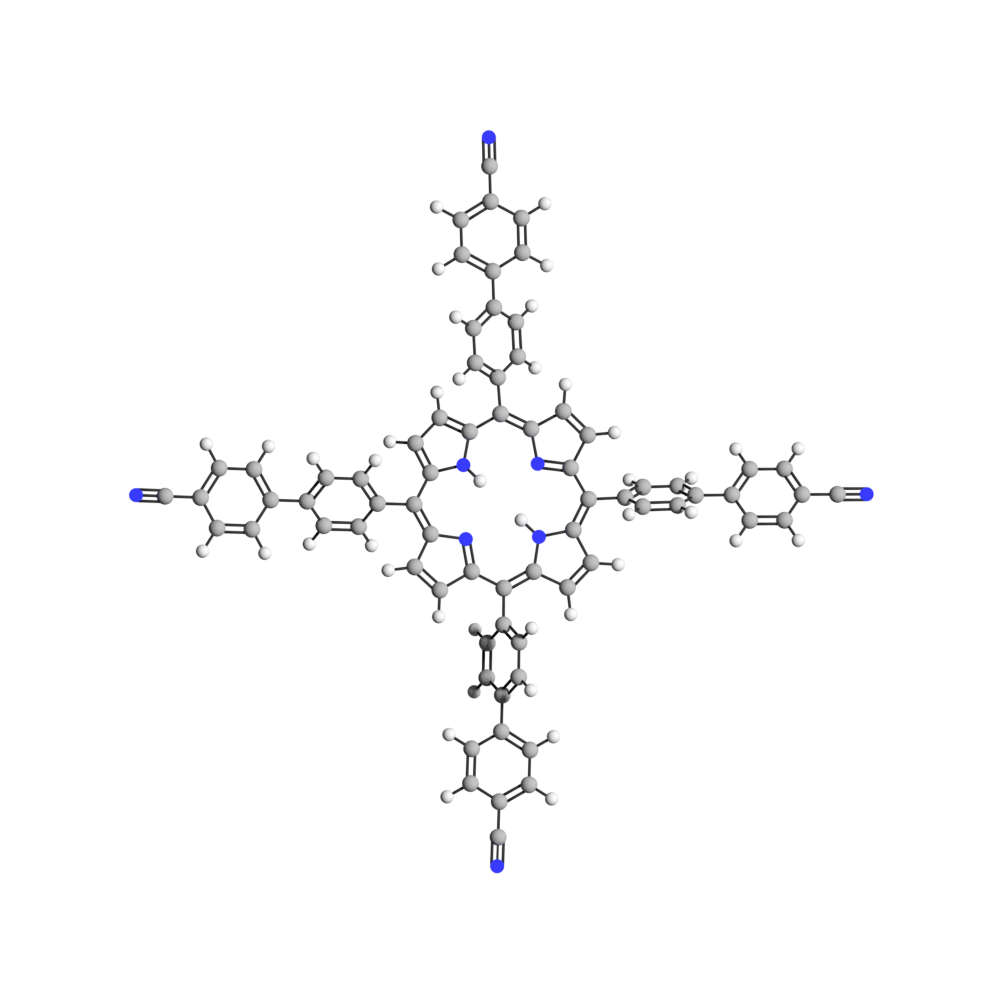
\includegraphics[width=0.3\textwidth]{./images/molecules/TPCN}
%	\caption{TPCN molecule}
%	\label{fig:TPCN}
%\end{figure}


%%%%%%%%%%%%%%%%%%%%%%%%%%%%%%%%%%%%%%%%%%%%%%%%%%%%%%%%%%%%%%%%%%%%%%%%%%%%%%%%%%%%%%%%%%%
%%%%%%%%%%%%%%%%%%%%%%%%%%%%%%%%%%%nitro-prophines%%%%%%%%%%%%%%%%%%%%%%%%%%%%%%%%%%%%%%%%%
\subsection{Porphine: [di-[tert-butyl]-phenyl)]-porphyrin derivatives}
\label{sec:TBP}\index{molecules!TBP}
\begin{itemize}
	\item[one-leg:]  	 5,10,15-Tri(3,5-di-tert-butylphenyl)-   20-(Nitrophenyl)porphyrine
	\item[two-leg cis:] 	5,10-Bis(3,5-di-tert-butylphenyl)-15,20-Bis(Nitrophenyl)porphyrine
	\item[two-leg trans:] 	5,15-Bis(3,5-di-tert-butylphenyl)-10,20-Bis(Nitrophenyl)porphyrine
\end{itemize}

\begin{figure}[h!]\centering
	\subfigure[Single functional group]{
		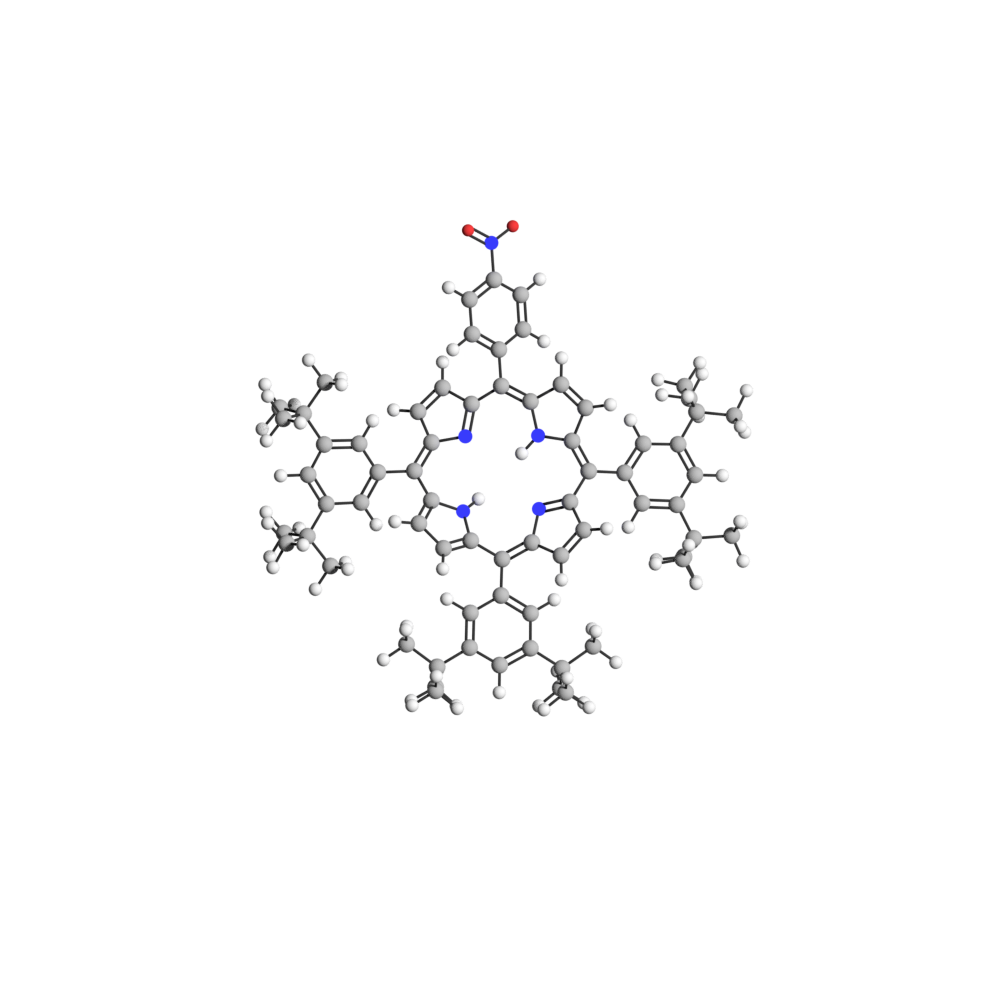
\includegraphics[angle=90, width=0.3\textwidth]{./images/molecules/TBP-single}
		\label{fig:TBP-single}
	} %
	\subfigure[Trans-configuration]{
		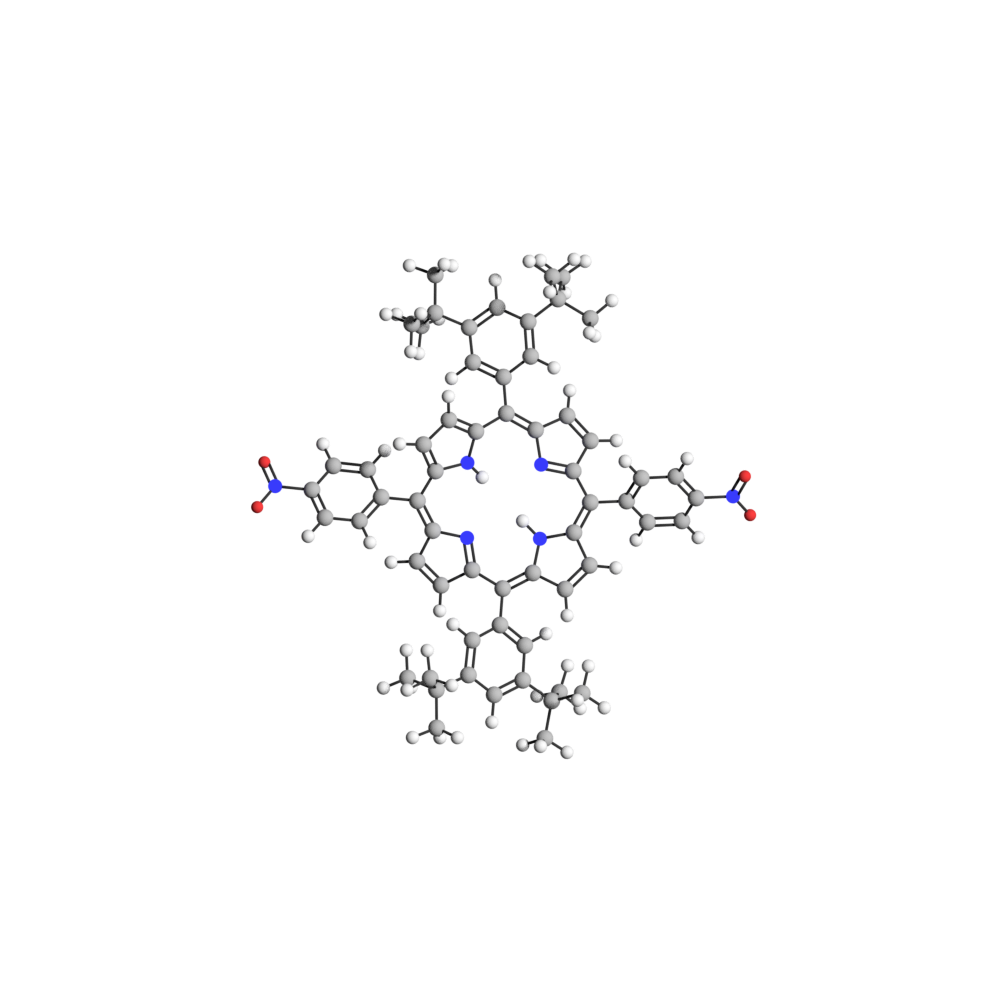
\includegraphics[angle=0, width=0.3\textwidth]{./images/molecules/TBP-trans}
		\label{fig:TBP-trans}
	} %
	\subfigure[Cis-configuration]{
		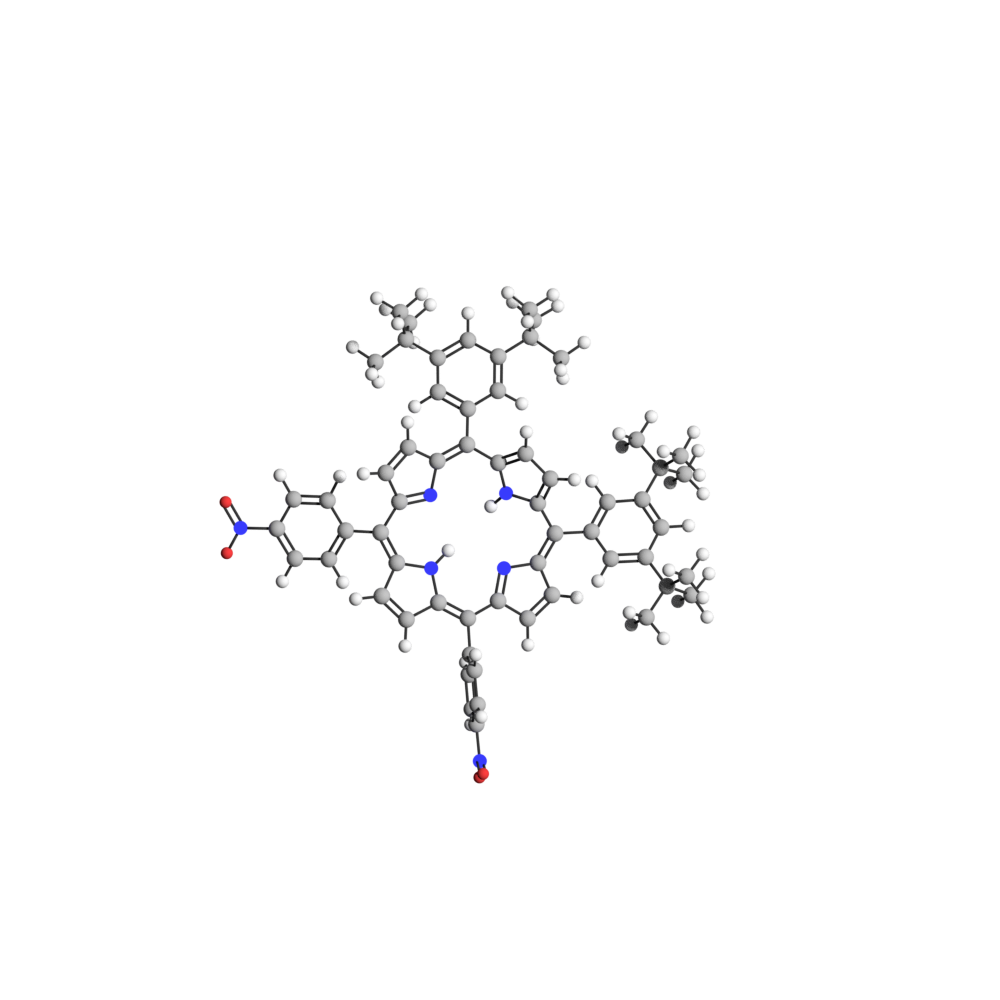
\includegraphics[angle=0, width=0.3\textwidth]{./images/molecules/TBP-cis}
		\label{fig:TBP-cis}
	} %
	\caption{Functionalized tert-butyl-phenyl-porphines. \subref{fig:TBP-single} shows a single functionalized porphine molecules. An additional function may be added in \subref{fig:TBP-cis} cis-  and \subref{fig:TBP-trans} position.}
	\label{fig:TBP}
\end{figure}	

Tetrapyrroles like porphyrins and phthalocyanines play important roles in biological systems \cite{battersby_tetrapyrroles_2000}. Both species are able to incorporate metal atoms that control the function. Not only are they interesting model systems to study interaction towards a (metallic) substrate\cite{auwarter_porphyrins_2015, auwarter_controlled_2007, diller_vacuo_2016}. Their use in metal-organic frameworks highlights the use of scientific knowledge to design "real world" sensor applications\cite{Lustig_Metal-organic_2017}. 


Tert-butyl functionals have been used in a variety of molecules \cite{moresco_conformational_2001}. Due to their bulky nature, they electronically decouple the porphyrin’s delocalized p-orbital system from the metallic surface just by lifting the molecule. They may undergo heavy conformational deformation when outer influences (like metalization of the central porphine core) act on the molecule \cite{stark_massive_2014}. Switching capabilities are well investigated \cite{loppacher_direct_2003} and it is possible to switch them with a voltage pulse through the STM tip \cite{ditze_energetics_2014}. Experiments with similar molecules investigate the heat-induced formation of 1D and 2D conglomerates on a Au(111) surface.\cite{pham_heat-induced_2015}

\begin{itemize}
	\item Free base nitrophenyl - 5,10,15 Tri [di-[tert-butyl]-phenyl)]-porphyrin \index{nitro porphin} has 3(2) di-tert-butyl-phenyl groups attached to the porphine macro cycle at the meso-positions of the molecule. The free meso-positions are occupied with nitrophenyl groups as shown in \autoref{fig:TBP-single} If more than one functional group is present, one can distinguish between trans (\autoref{fig:TBP-trans}) and cis configuration (\autoref{fig:TBP-cis}), whether the two functional groups are opposite or neighboring.
	\item The appearance of STM data is correlated to the molecular configuration according to \cite{mishra_current-driven_2015} meaning that the lobes consisting of (3,5-di-tert-butylphenyl) are imaged as bright protrusions, while the functional nitro group is imaged fainter. This holds true for cis- and trans-substituted molecules\cite{yokoyama_selective_2001}.
	\item Tert-butyl groups can rotate to form flexible legs. Interaction with the substrate results in adsorption-induced conformational changes.\cite{ecija_dynamics_2016}
\end{itemize}
Drawings for various functional groups and molecules can be found in \cite{jorgensen_salem_1973}.
\textcolor{red}{\textbf{DIPOLE, ref section}}
%%%%%%%%%%%%%%%%%%%%%%%%%%%%%%%%%%%%%%%%%%%%%%%%%%%%%%%%%%%%%%%%%%%%%%%%%%%%%%%%%%%%%%%%%%%
	%%%%%%%%%%%%%%%%%%%%%%%%%%%%%%%%%%%	helicenes %%%%%%%%%%%%%%%%%%%%%%%%%%%%%%%%%%%%%%%%%
	\subsection{Helicene: Cyano functionalization of helicenes}
	\label{sec:helicene}\index{molecules!Helicene}
	\begin{itemize}
		\item[Dicyano-dibenzo-[5]helicene]: 7,8-Bis(cyano)-Dibenzo-helicene
	\end{itemize}
	
	\begin{figure}[h!]
		\centering
		\subfigure[Top view]{
			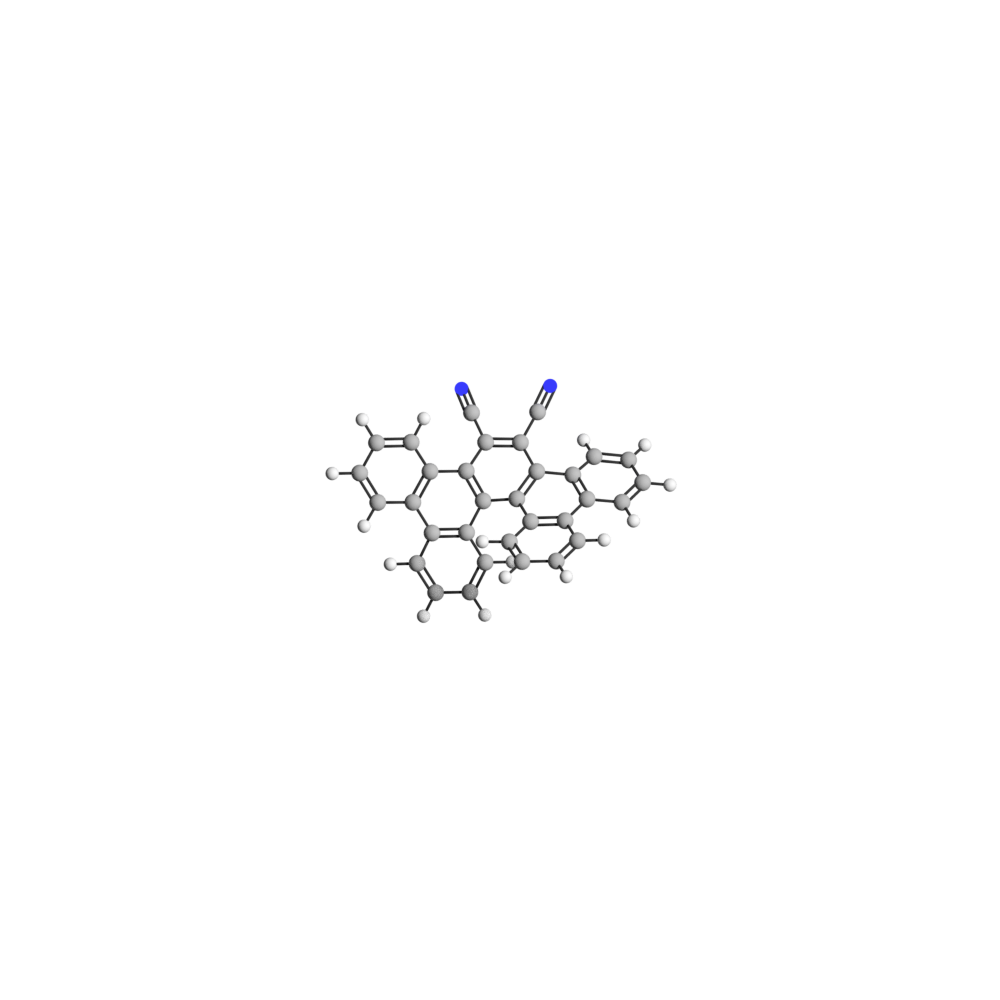
\includegraphics[width=0.3\textwidth]{./images/molecules/helicene}
			\label{fig:helicene-top}
		} \quad
		\subfigure[Side view]{
			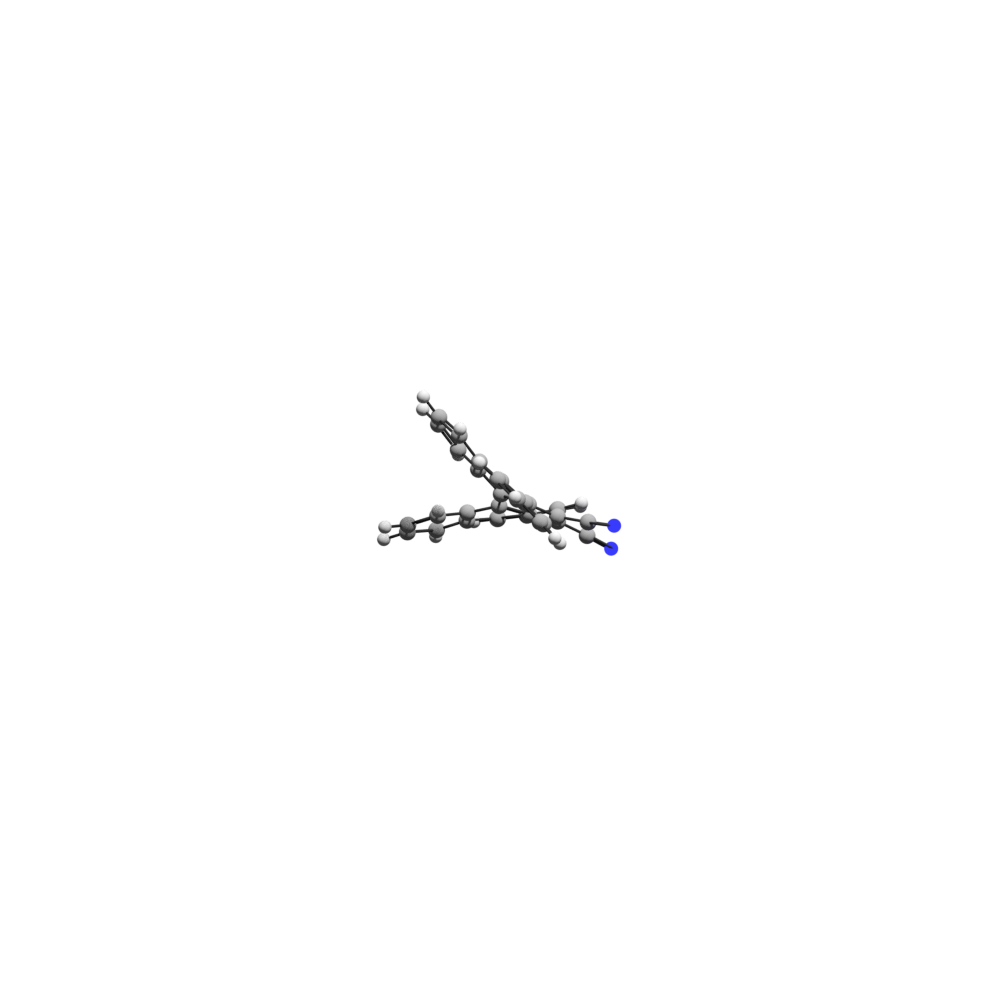
\includegraphics[width=0.3\textwidth]{./images/molecules/helicene-side}
			\label{fig:helicene-side}
		} \quad
		\caption{DCDB. \subref{fig:helicene-top} Top view, \subref{fig:helicene-side} side view}
		\label{fig:helicene}
	\end{figure}
	
	Helicenes were first synthezised in the 1950's \cite{Newman_synthesis_1956}. They consist of ortho condensed carbon rings that form a spiral due to overcrowding in their center. While they first drew attention due to their fluorescence properties \cite{vander_donckt_fluorescence_1968}, helicenes are interesting molecules because of their chiral feature. Two different turn directions exist, left and right.  
	
	In this work we investigate sub-monolayer coverages of 7,8-dicyano-5,6,9,10-dibenzo-[5]Helicene (dcdb-[5]H). The benzol groups condensed at positions 5,6,9,10 to the five carbon rings of [5]H (db-[5]H) are used to achieve a more distinct footprint of the molecule. Two cyano groups added at the central carbon ring induce a permanent dipole moment of 6.3 D (\autoref{fig:hel-fig1}a,b) and complete the molecule we use here. 

	For more information, please refer to \autoref{section:helicene}.